\section{Introduction}

\subsection[Mobile industry]{The mobile industry}

\begin{frame}
    \frametitle{The mobile industry and its operating systems}
    \centering

    Android 1.0 was released in September 2008 (10 years ago)

    \vspace{-5pt}

    \begin{figure}[!ht]
        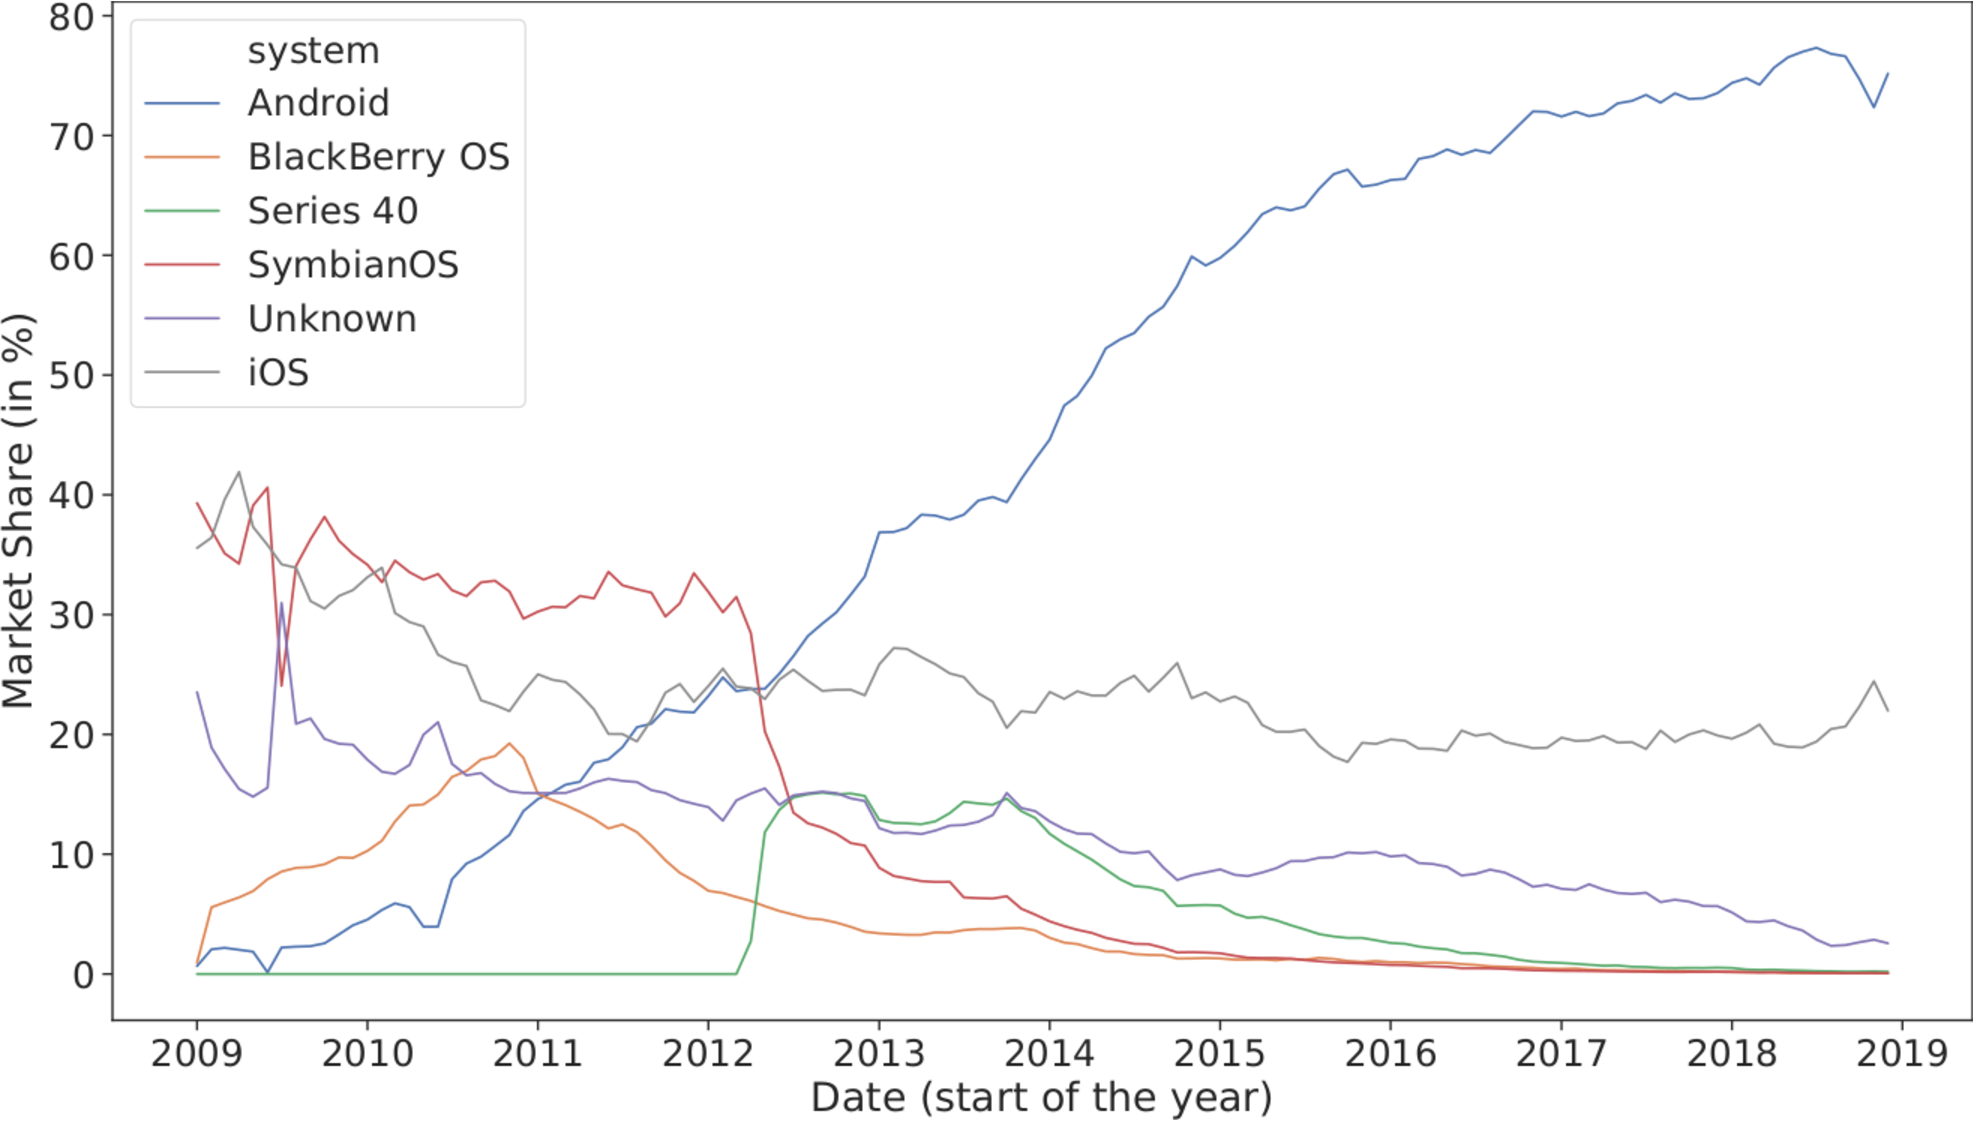
\includegraphics[width=0.9\textwidth]{figures/introduction/shares.pdf}
        \caption{\footnotesize{Market shares of mobile operating systems (source: StatCounter)}}
    \end{figure}

    \vspace{-15pt}

    There are now more than \textbf{2 billion} active Android devices
    \smallskip{}
    \scriptsize{}
    source: Android Security \& Privacy 2018 Year In Review


\end{frame}

\begin{frame}
    \frametitle{The mobile industry and its actors}
    \centering

    Google Play includes \textbf{2.1 million} Android applications \\
    \smallskip{}
    \scriptsize{}
    source: Number of apps available in leading app stores as of Q1 2019, Statista

    \begin{figure}[!ht]
        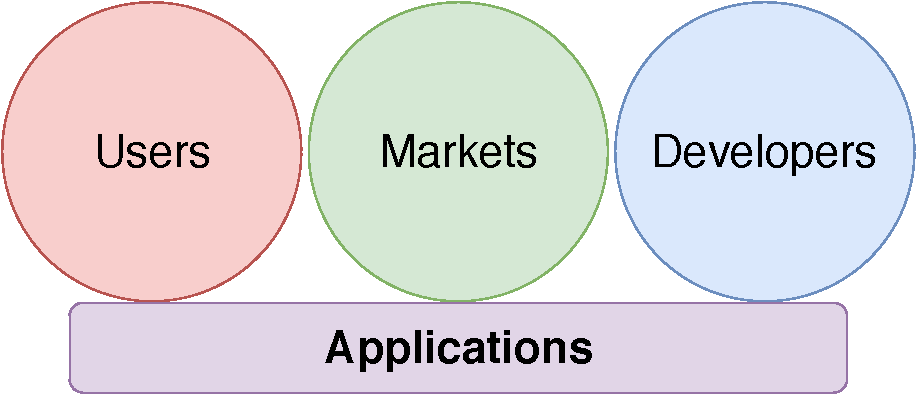
\includegraphics[width=0.8\textwidth]{figures/introduction/actors.pdf}
    \end{figure}

    \normalsize{}
    Google Play Protect scans over \textbf{50 billion} APKs each day \\
    \smallskip{}
    \scriptsize{}
    source: Android Security \& Privacy 2018 Year In Review

\end{frame}

\begin{frame}
    \frametitle{The mobile industry and its risks (1/2)}

    \medskip{}

    \begin{figure}[!ht]
        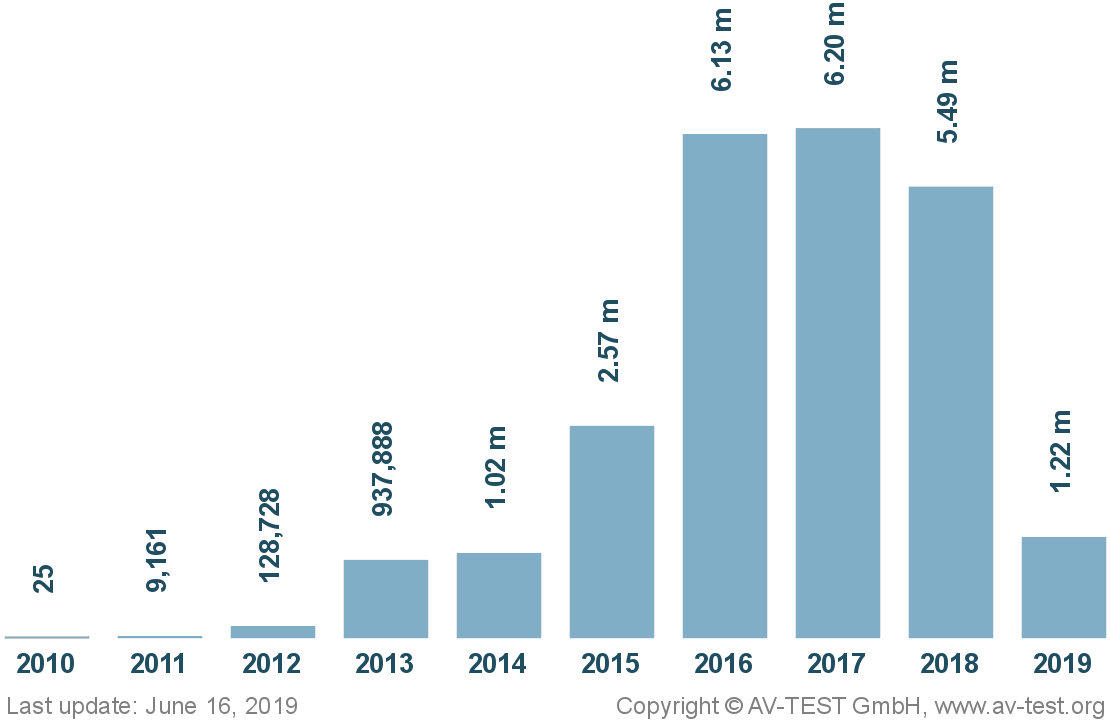
\includegraphics[width=0.95\textwidth]{figures/introduction/evolution.png}
        \caption{\scriptsize{Registrations of new Android malware from 2010 to 2019 (source: AV-TEST)}}
    \end{figure}

\end{frame}

\begin{frame}
    \frametitle{The mobile industry and its risks (2/2)}
    \centering

    \begin{figure}[!ht]
        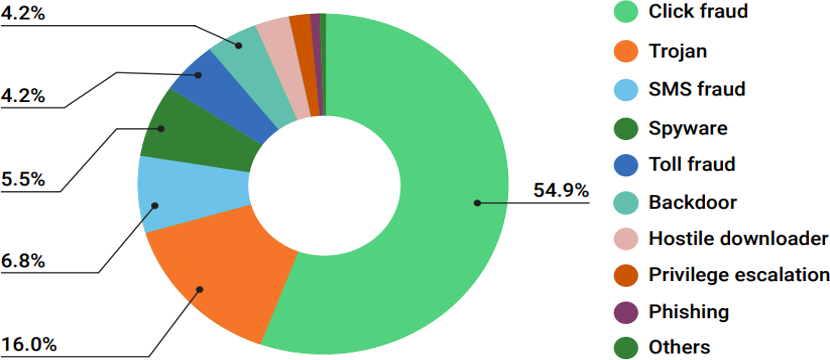
\includegraphics[height=0.32\textheight]{figures/introduction/categories/play.png}
        \caption{\scriptsize{Distribution of malware categories in Google Play}}
    \end{figure}

    \vspace{-20pt}

    \begin{figure}[!ht]
        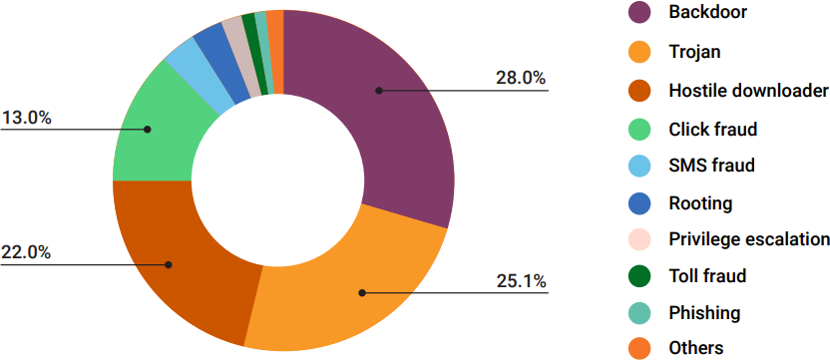
\includegraphics[height=0.32\textheight]{figures/introduction/categories/others.png}
        \caption{\scriptsize{Distribution of malware categories outside of Google Play}}
    \end{figure}

    \vspace{-10pt}

    \scriptsize{source: Android Security \& Privacy 2018 Year In Review}

\end{frame}

\subsection[Android security]{The security of Android}

\begin{frame}
    \frametitle{How to improve the security of Android}

    \begin{tabularx}{\textwidth}{l r}
        \multicolumn{2}{c}{\textbf{Challenge 1:~Definition of Android malware}\vspace{5pt}} \\
        \textbullet \dotline{300pt} & \\
        \textbullet \dotline{300pt} & \\
        \textbullet \dotline{300pt} & \\
        \\
        \multicolumn{2}{c}{\textbf{Challenge 2:~Detection of Android malware}\vspace{5pt}} \\
        \textbullet \dotline{300pt} & \\
        \textbullet \dotline{300pt} & \\
        \textbullet \dotline{300pt} & \\
        \\
        \multicolumn{2}{c}{\textbf{Challenge 3:~Comprehension of Android malware}\vspace{5pt}} \\
        \textbullet \dotline{300pt} & \\
        \textbullet \dotline{300pt} & \\
        \textbullet \dotline{300pt} & \\
    \end{tabularx}

\end{frame}

\begin{frame}
    \frametitle{Challenge 1:~Definition of Android malware}

    \begin{columns}
        \begin{column}{0.8\textwidth}
            \begin{block}{}
                \centering
                \textbf{Context}
            \end{block}
            \begin{itemize}
                \item Malware is loosely defined as harmful software
                \item Human expertise is crucial to qualify malware
            \end{itemize}

            \begin{block}{}
                \centering
                \textbf{Problems}
            \end{block}
            \begin{itemize}
                \item There is a global shortage of security experts
                \item Computers need precise definitions to operate
            \end{itemize}

            \begin{block}{}
                \centering
                \textbf{Objectives}
            \end{block}
            \begin{itemize}
                \item Gather information from past human decisions
                \item Provide a more precise definition with artifacts
            \end{itemize}
        \end{column}

        \begin{column}{0.3\textwidth}
            \begin{figure}[!ht]
                
\includegraphics[width=0.95\textwidth]{figures/introduction/definition.jpg}
            \end{figure}
        \end{column}
    \end{columns}

\end{frame}

\begin{frame}
    \frametitle{Challenge 2:~Detection of Android malware}

    \begin{columns}
        \begin{column}{0.3\textwidth}
            \begin{figure}[!ht]
                
\includegraphics[width=0.8\textwidth]{figures/introduction/detection.jpg}
            \end{figure}
        \end{column}

        \begin{column}{0.8\textwidth}
            \begin{block}{}
                \centering
                \textbf{Context}
            \end{block}
            \begin{itemize}
                \item Malware authors already rely on automation
                \item Machine learning ``protects'' our infrastructure
            \end{itemize}

            \begin{block}{}
                \centering
                \textbf{Problems}
            \end{block}
            \begin{itemize}
                \item The representativity of malware sets is crucial
                \item Machine learning requires vast amount of data
            \end{itemize}

            \begin{block}{}
                \centering
                \textbf{Objectives}
            \end{block}
            \begin{itemize}
                \item Verify the quality of malware ground truths
                \item Provide larger ground truths for experiments
            \end{itemize}
        \end{column}
    \end{columns}

\end{frame}

\begin{frame}
    \frametitle{Challenge 3:~Comprehension of Android malware}

    \begin{columns}
        \begin{column}{0.8\textwidth}
            \begin{block}{}
                \centering
                \textbf{Context}
            \end{block}
            \begin{itemize}
                \item Android applications are extremely complex
                \item Dissecting an application is time-consuming
            \end{itemize}

            \begin{block}{}
                \centering
                \textbf{Problems}
            \end{block}
            \begin{itemize}
                \item A malware analysis produces too much data
                \item There is a global lack of information sharing
            \end{itemize}

            \begin{block}{}
                \centering
                \textbf{Objectives}
            \end{block}
            \begin{itemize}
                \item Help security experts during their investigation
                \item Unify the content of ground truth descriptions
            \end{itemize}
        \end{column}

        \begin{column}{0.3\textwidth}
            \begin{figure}[!ht]
                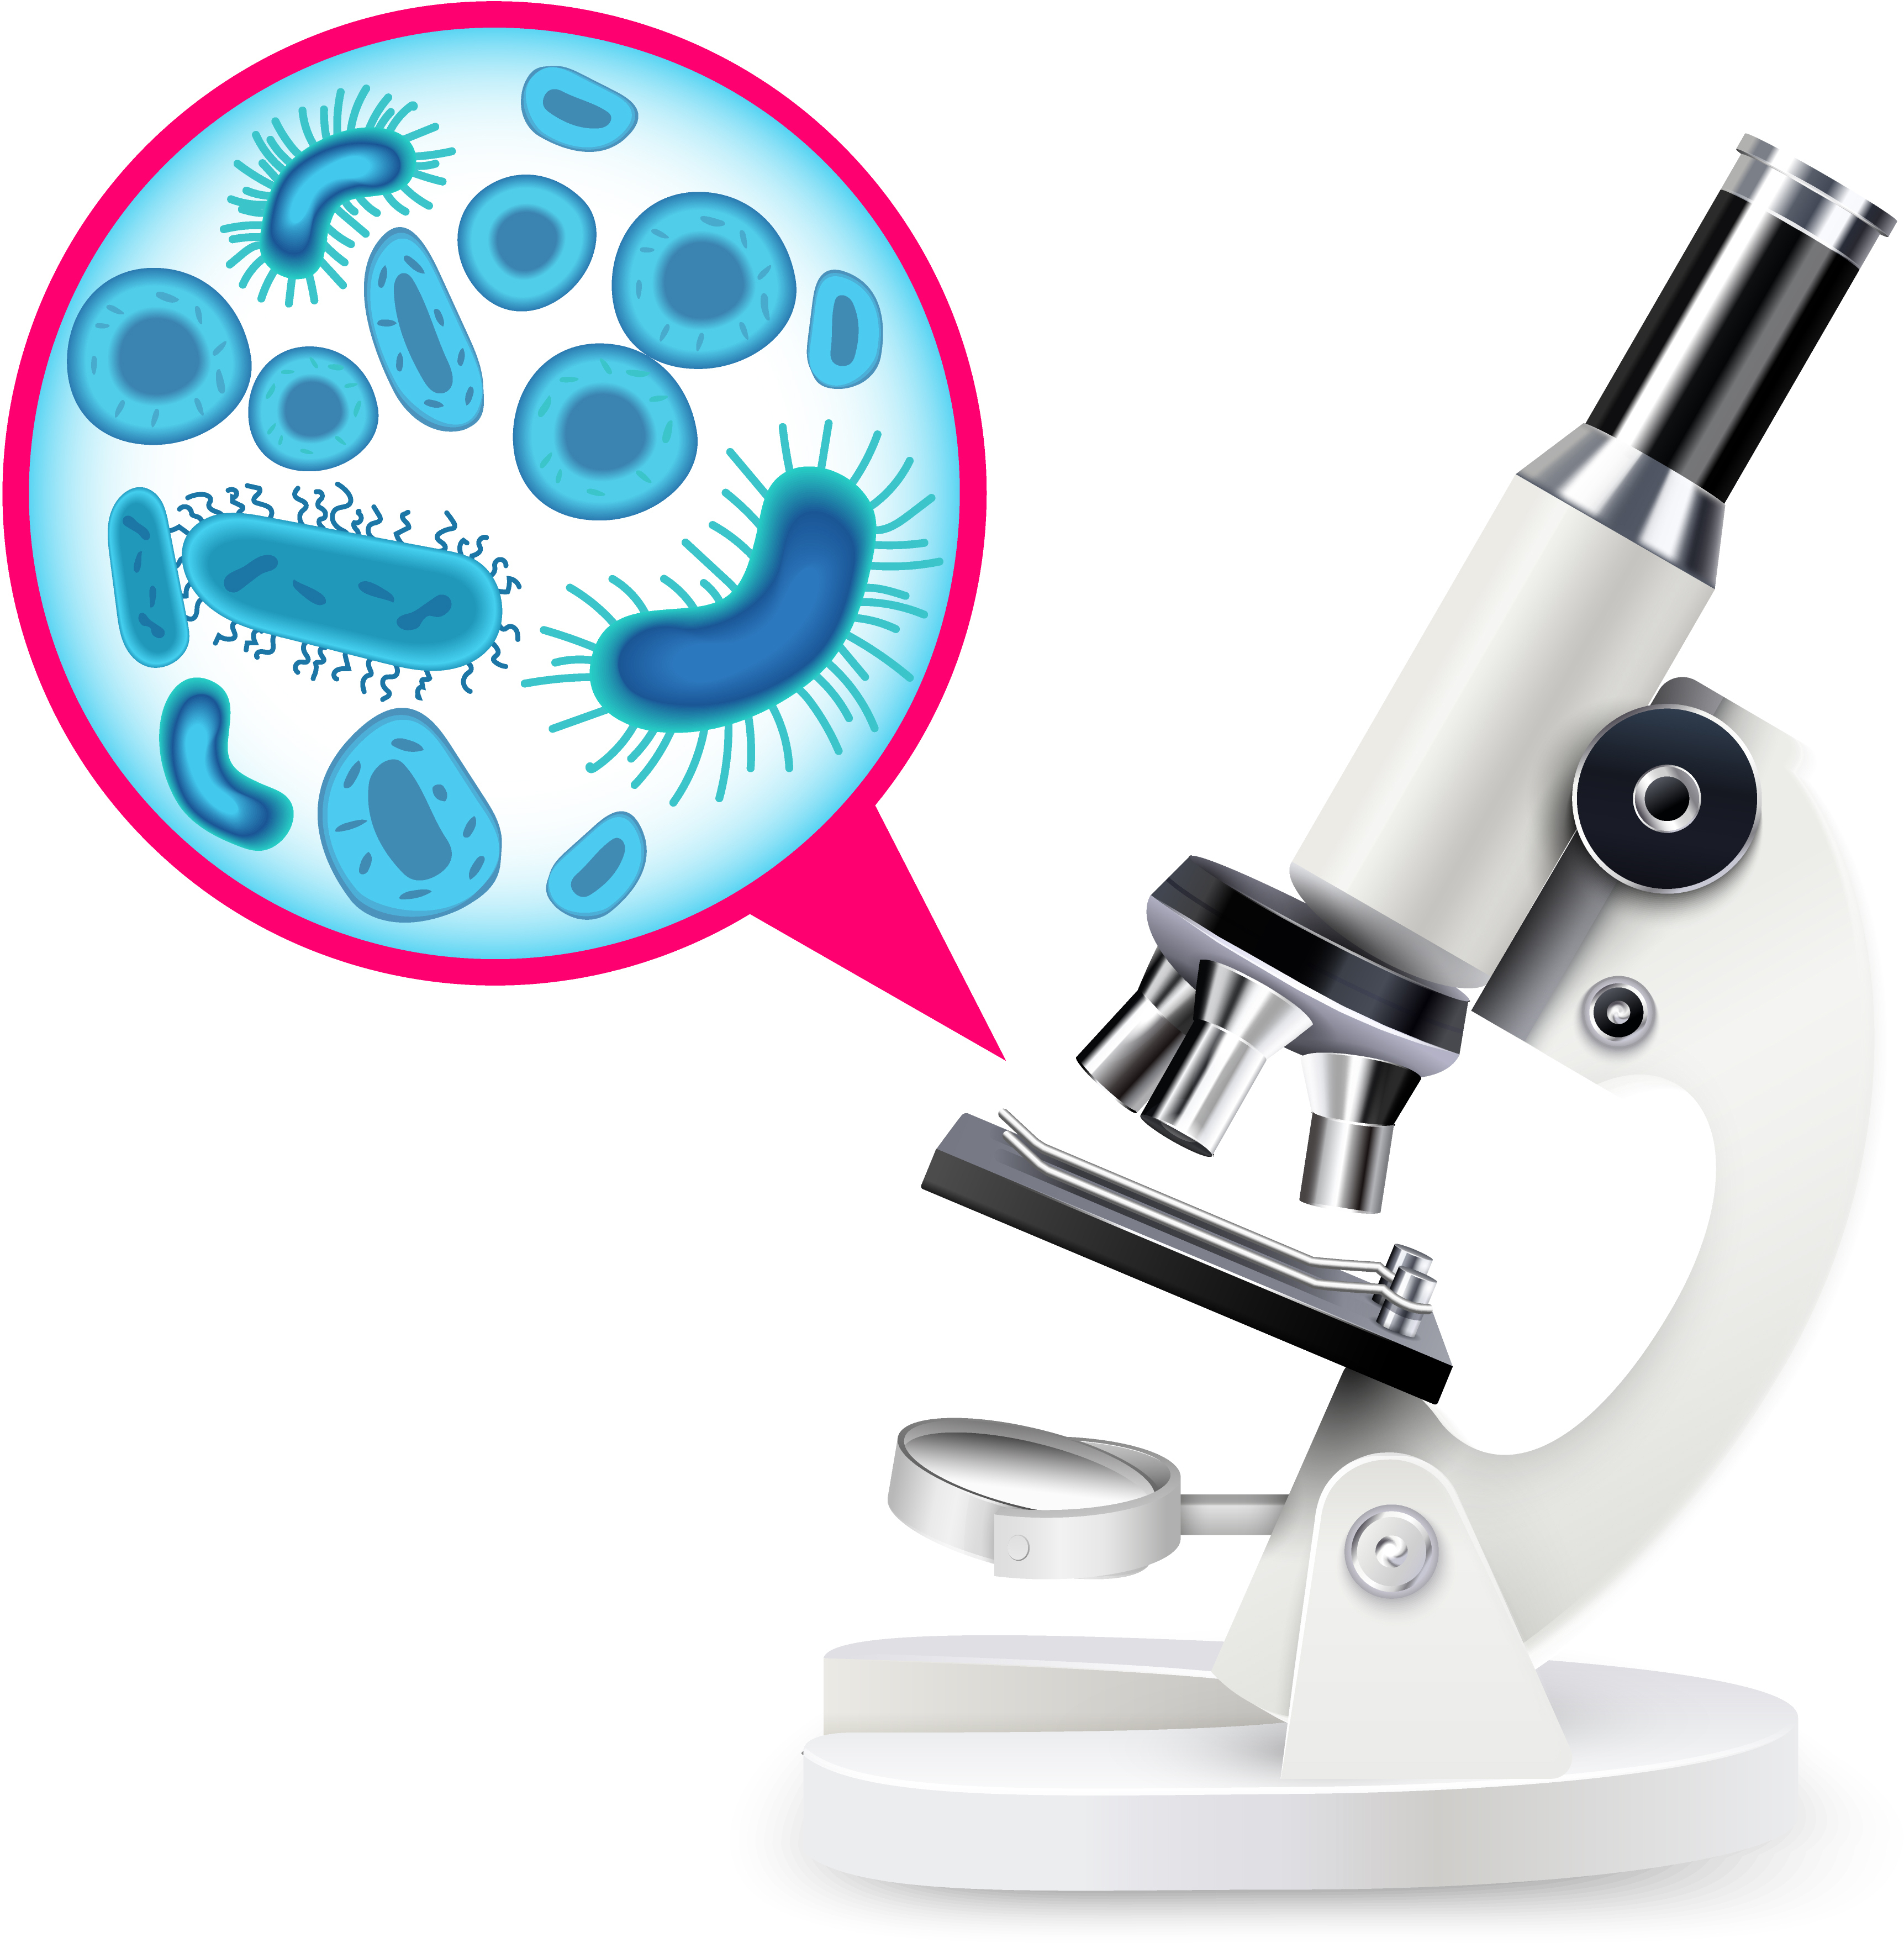
\includegraphics[width=0.95\textwidth]{figures/introduction/comprehension.jpg}
            \end{figure}
        \end{column}
    \end{columns}

\end{frame}
